%!TEX root = main.tex
 %\section{System-level Participatory Design Findings\label{sec:pd_findings}}
 % From loaded tgn, generate latex from https://www.tablesgenerator.com/latex_tables/ 
% replace 
% $\sim$ --> ~
% $\textbackslash{}$ --> \
% \{ --> {
% \} --> }
\begin{table*}[ht!]
\centering
  \resizebox{0.95\textwidth}{!}{%
\begin{tabular}{|p{0.05cm}|l|l|l|l|l|}
	\hline
	                                                    & Component                                                                                                 & Feature                                                                                                              & Purpose                                                                                                                                                                                                      & Task Example                                                                                                                                                                                                                                                    & \begin{tabular}[c]{@{}l@{}}Similar Features\\ in Past VQSs\end{tabular}                                                                                                                                                                                         \\ \hline
	\rowcolor[HTML]{AADFFD} 
	\cellcolor[HTML]{AADFFD}                                   & \cellcolor[HTML]{AADFFD}                                                                                  & \begin{tabular}[c]{@{}l@{}}Query by Sketch\\ (Figure \ref{zvOverview}B1)\end{tabular}               & \begin{tabular}[c]{@{}l@{}}Freehand sketching for \\ specifying pattern query.\end{tabular}                                                                                                                  & \begin{tabular}[c]{@{}l@{}}\A Find patterns with a peak \\ and long-tail decay that\\ may be supernovae candidates.\end{tabular}                                                                                                                 & \begin{tabular}[c]{@{}l@{}}All include sketch \\ canvas except~\cite{Hochheiser2004}.\end{tabular}                                                                                                                                        \\ \cline{3-6} 
	\rowcolor[HTML]{AADFFD} 
	\cellcolor[HTML]{AADFFD}                                   & \cellcolor[HTML]{AADFFD}                                                                                  & \begin{tabular}[c]{@{}l@{}}Input Equation\\ (Figure \ref{zvOverview}A1)\end{tabular}                & \begin{tabular}[c]{@{}l@{}}Specify a exact functional \\ form as a pattern query \\ (e.g., y=$x^2$).\end{tabular}                                                                                            & \begin{tabular}[c]{@{}l@{}}\M Find patterns exhibiting \\ inversely proportional \\ chemical relationship.\end{tabular}                                                                                                                          & ----                                                                                                                                                                                                                                                            \\ \cline{3-6} 
	\rowcolor[HTML]{AADFFD} 
	\cellcolor[HTML]{AADFFD}                                   & \multirow{-5}{*}{\cellcolor[HTML]{AADFFD}\begin{tabular}[c]{@{}l@{}}\textbf{Pattern Specification:}\\\textit{What is the shape of}\\\textit{the pattern query?}\end{tabular}} & \begin{tabular}[c]{@{}l@{}}Pattern Upload\\ (Figure \ref{zvOverview}D2)\end{tabular}                & \begin{tabular}[c]{@{}l@{}}Upload a pattern consisting\\ of a sequence of points as \\ a query.\end{tabular}                                                                                                 & \begin{tabular}[c]{@{}l@{}}\A Find supernovae based on \\ previously discovered sources.\end{tabular}                                                                                                                                            & \begin{tabular}[c]{@{}l@{}}Upload CSV\\ \cite{mohebbi2011google}\end{tabular}                                                                                                                                                                  \\ \cline{2-6} 
	\rowcolor[HTML]{AADFFD} 
	\cellcolor[HTML]{AADFFD}                                   & \cellcolor[HTML]{AADFFD}                                                                                  & \begin{tabular}[c]{@{}l@{}}Smoothing\\ (Figure \ref{zvOverview}D2)\end{tabular}                     & \begin{tabular}[c]{@{}l@{}}Interactively adjusting the level \\ of denoising on visualizations,\\ effectively changing the degree\\ of shape approximation when \\ performing pattern matching.\end{tabular} & \begin{tabular}[c]{@{}l@{}}\textbf{A, M:} Eliminate patterns \\ matched to spurious noise.\end{tabular}                                                                                                                                        & \begin{tabular}[c]{@{}l@{}}Smoothing ~\cite{Mannino2018}\\ Angular slope queries ~\cite{Hochheiser2004}\\ Trend querylines ~\cite{ryall2005querylines}\end{tabular}                     \\ \cline{3-6} 
	\rowcolor[HTML]{AADFFD} 
	\cellcolor[HTML]{AADFFD}                                   & \cellcolor[HTML]{AADFFD}                                                                                  & \begin{tabular}[c]{@{}l@{}}Range \\ Selection\\ (Figure \ref{zvOverview}B2, D4)\end{tabular}        & \begin{tabular}[c]{@{}l@{}}Restrict to query only in \\ specific x/y ranges of interest \\ through brushing selected\\ x-range and filtering \\ selected y-range.\end{tabular}                               & \begin{tabular}[c]{@{}l@{}}\A Matching only around \\ shape exhibiting a peak.\\ \M Matching only around \\ shape region that exhibit linear\\ or exponential relationships\end{tabular}                                          & \begin{tabular}[c]{@{}l@{}}Text Entry ~\cite{wattenberg2001sketching,Mannino2018}\\ Min/max boundaries ~\cite{ryall2005querylines}\\ Range Brushing ~\cite{Hochheiser2001}\end{tabular} \\ \cline{3-6} 
	\rowcolor[HTML]{AADFFD} 
	\multirow{-20}{*}{\cellcolor[HTML]{AADFFD}\rot{\vspace{-2pt}Top-Down}}         & \multirow{-10}{*}{\cellcolor[HTML]{AADFFD}\begin{tabular}[c]{@{}l@{}}\textbf{Match Specification:}\\\textit{How should the pattern}\\\textit{query be matched} \\\textit{with other visualizations?}\end{tabular}}   & \begin{tabular}[c]{@{}l@{}}Range \\ Invariance\\ (Figure \ref{zvOverview}D1,4)\end{tabular}         & \begin{tabular}[c]{@{}l@{}}Ignoring vertical or horizontal \\ differences in pattern matching \\ through option for x-range\\ normalization and y-invariant\\ similarity metrics .\end{tabular}              & \begin{tabular}[c]{@{}l@{}}\A Searching for existence of a\\ peak above a certain amplitude.\\ \G Searching for a \\ ``generally-rising" pattern.\end{tabular}                                                                    & \begin{tabular}[c]{@{}l@{}}Temporal invariants ~\cite{correll2016semantics}\end{tabular}                                                                                                                                                \\ \hline
	\rowcolor[HTML]{FBE39C} 
	\cellcolor[HTML]{FBE39C}                                   & \cellcolor[HTML]{FBE39C}                                                                                  & \begin{tabular}[c]{@{}l@{}}Data selection\\ (Figure \ref{zvOverview}A)\end{tabular}                 & \begin{tabular}[c]{@{}l@{}}Changing the collection of \\ visualizations to iterate over.\end{tabular}                                                                                                        & \begin{tabular}[c]{@{}l@{}}\M Explore tradeoffs and \\ relationships between \\ physical attributes.\end{tabular}                                                                                                                                & ----                                                                                                                                                                                                                                                            \\ \cline{3-6} 
	\rowcolor[HTML]{FBE39C} 
	\cellcolor[HTML]{FBE39C}                                   & \multirow{-4}{*}{\cellcolor[HTML]{FBE39C}\begin{tabular}[c]{@{}l@{}}\textbf{View Specification:} \\ \textit{What data to visualize} \\ \textit{and how should it} \\ \textit{be displayed?}\end{tabular}}    & \begin{tabular}[c]{@{}l@{}}Display control\\ (Figure \ref{zvOverview}D4)\end{tabular}               & \begin{tabular}[c]{@{}l@{}}Changing the details of \\ how visualizations should\\ be displayed.\end{tabular}                                                                                                 & \begin{tabular}[c]{@{}l@{}}\M Non-time-series data should \\ be displayed as scatterplot.\end{tabular}                                                                                                                                           & ----                                                                                                                                                                                                                                                            \\ \cline{2-6} 
	\rowcolor[HTML]{FBE39C} 
	\cellcolor[HTML]{FBE39C}                                   & \cellcolor[HTML]{FBE39C}                                                                                  & \begin{tabular}[c]{@{}l@{}}Filter\\ (Figure \ref{zvOverview}D3)\end{tabular}                        & \begin{tabular}[c]{@{}l@{}}Display and query only on data \\ that satisfies the composed \\ filter constraints.\end{tabular}                                                                                 & \begin{tabular}[c]{@{}l@{}}\A Eliminate unlikely \\ candidates by navigating to \\ more probable data regions.\\ \textbf{M, G:} Compare how overall\\ patterns change when filtered \\ to particular data subsets.\end{tabular} & ----                                                                                                                                                                                                                                                            \\ \cline{3-6} 
	\rowcolor[HTML]{FBE39C} 
	\multirow{-10}{*}{\cellcolor[HTML]{FBE39C}\rot{\vspace{-2pt}Context Creation}} & \multirow{-7}{*}{\cellcolor[HTML]{FBE39C}\begin{tabular}[c]{@{}l@{}}\textbf{Slice-and-Dice:} \\ \textit{How does navigating} \\ \textit{to another data subset} \\ \textit{change the query result?}\end{tabular}}                                                  & \begin{tabular}[c]{@{}l@{}}Dynamic Class \\ (Figure~\ref{dcc})\end{tabular}                    & \begin{tabular}[c]{@{}l@{}}Create custom classes of data \\ that satisfies one or more \\ specified range constraints. \\ Display aggregate \\ visualizations for separate\\ data classes.\end{tabular}      & \begin{tabular}[c]{@{}l@{}}\textbf{A, M:} Examine aggregate \\ patterns of different data \\ classes.\end{tabular}                                                                                                                             & ----                                                                                                                                                                                                                                                            \\ \hline
	\rowcolor[HTML]{B5E1A4} 
	\cellcolor[HTML]{B5E1A4}                                   & \begin{tabular}[c]{@{}l@{}}\textbf{Result Querying:} \\ \textit{What other visualizations}\\ \textit{``look similar" to the} \\\textit{selected pattern?}\end{tabular}                                                & \begin{tabular}[c]{@{}l@{}}Drag-and-drop\\ (Figure \ref{zvOverview}C, E)\end{tabular}               & \begin{tabular}[c]{@{}l@{}}Querying with any selected\\ result visualization as pattern\\ query (either from \\ recommendations or results).\end{tabular}                                                    & \begin{tabular}[c]{@{}l@{}}\textbf{A, G, M:} Find other objects that\\ are similar to X; Examine what \\ other objects similar to X look \\ like overall.\end{tabular}                                                                         & \begin{tabular}[c]{@{}l@{}}Drag-and-drop ~\cite{Hochheiser2001}\\ Double-Click ~\cite{correll2016semantics}\end{tabular}                                                                                        \\ \cline{2-6} 
	\rowcolor[HTML]{B5E1A4} 
	\multirow{-6}{*}{\cellcolor[HTML]{B5E1A4}\rot{\vspace{-2pt}Bottom-Up}}        & \begin{tabular}[c]{@{}l@{}}\textbf{Recommendation:} \\ \textit{What are the key patterns} \\ \textit{in this dataset?}\end{tabular} & \begin{tabular}[c]{@{}l@{}}Representative \\ and Outliers\\ (Figure \ref{zvOverview}E)\end{tabular} & \begin{tabular}[c]{@{}l@{}}Displaying visualizations of \\ representative trends and outlier\\ instances based on clustering.\end{tabular}                                                                   & \begin{tabular}[c]{@{}l@{}}\A Examine anomalies and debug \\ data errors through outliers.\\ \textbf{G, M:} Understand representative \\ trends common to this dataset \\ (or filtered subset).\end{tabular}                    & ----                                                                                                                                                                                                                                                            \\ \hline
\end{tabular}
}
  \caption{\rchange{Taxonomy of key capabilities essential to VQSs and major features incorporated via participatory design. We organize each feature based on its functional component. From left to right, each of the three sensemaking process (first column) is broken down into key functional components (second column) in VQSs. Each component addresses a pro-forma question from a system's perspective.} Table cells are further colored according to the sensemaking process that each component corresponds to (Blue: Top-down, Yellow: Context creation, Green: Bottom-up). We list the functional purpose of each feature based on how it is implemented in \zvpp, example use cases from participatory design (\A astronomy, \M material science, \G genetics), and similar features incorporated in past VQSs. Given the exhaustive nature of Table~\ref{bigfeaturetable}, each motivated by example use cases from one or more domains, we further organize the features in terms of the Section~\ref{sec:sensemaking} sensemaking framework and assess their effectiveness in the Section~\ref{sec:eval_findings} evaluation study.}\label{bigfeaturetable}
  \vspace*{-15pt}
\end{table*}
 \section{\rchange{Co-design} Process and System Overview\label{sec:pd_findings}}
%All of the three domains described in the previous section recognized the need for a VQS. As discussed in Section~\ref{sec:methods},
%we worked closely with participants to develop features to address their problems and challenges.
 Given the need for a VQS highlighted via contextual \rchange{inquiry}, we further collaborated with participants to develop features to address their problems and challenges \rchange{in Phase II of our study}. In this section, we first reflect on our feature discovery process to introduce our \rchange{design findings}, then we provide a high-level system overview of the \rchange{design} product, \zvpp.
 \subsection{The Collaborative Feature Discovery Process~\label{sec:feature_dsicovery}}
 \par Throughout the \rchange{design} process, we worked closely with participants to discover VQS capabilities that were essential for addressing their high-level domain challenges. We identified various subtasks based on the participant's workflow, designed sensible features for accomplishing these subtasks that could be used in conjunction with existing VQS capabilities, and elicited feedback on intermediate feature prototypes. Bodker et al.~\cite{BodkerGronbaek} cite the importance of encouraging user participation and creativity in cooperative design through different techniques, such as future workshops, critiques, and situational role-playing. Similarly, our \cut{PD} objective was to collect as many feature proposals as possible, while being inclusive across different domains. We further organized these features into Table~\ref{bigfeaturetable} through an iterative coding process by one of the authors.
 \par In grounded theory methods~\cite{Muller2012}, researchers first create \emph{open codes} to assign descriptive labels to raw data, followed by grouping open codes together by relationships or categories to form \emph{axial codes}. Finally, \emph{selective codes} are obtained by focusing on specific sets of axial codes to come up with a set of core emerging concepts. Inspired by grounded theory methods, we first collected the list of features and example usage scenarios \cut{from PD} and similar capabilities in existing VQSs as open codes\rchange{, corresponding to individual rows in Table~\ref{bigfeaturetable}}. Then, we further organized this list into axial codes representing ``components''\rchange{: core functionalities that are essential in VQSs (second} column in Table~\ref{bigfeaturetable}). Finally, \cut{as we will describe in Section~\ref{sec:sensemaking}, }the selective codes capture each of the sensemaking processes (\rchange{leftmost column} in Table~\ref{bigfeaturetable}). Instead of describing this table in detail, we present a typical example of how this table is organized. Consider \rchange{the row corresponding to the Smoothing feature in} Table~\ref{bigfeaturetable}: one of the common challenges in astronomy and material science is that noise in the dataset can result in large numbers of false-positive matches. To address this issue, smoothing is a feature in \zvpp that enables users to adjust data smoothing algorithms and parameters on-the-fly to both denoise the data and change the degree of shape approximation applied to all visualizations when performing pattern matching. %smoothing is a feature in \zvpp that enables users to adjust data smoothing algorithms and parameters on-the-fly to both denoise the data and change the degree of shape approximation applied to all visualizations when performing pattern matching. This is useful for domains such as astronomy and material science where the dataset is noisy with large numbers of false positives that could be matched to any given pattern query. 
 Smoothing, along with range selection and range invariance \cut{(row 5 and 6)}, is part of the \emph{match specification} component: VQS mechanisms for clarifying how matching should be performed. Both match specification and \emph{pattern specification} (a description of what the pattern query should look like) are essential components for supporting the sensemaking process top-down pattern search (in blue).%, described in Section~\ref{sec:sensemaking}.
 % Smoothing is also supported in Qetch~\cite{Mannino2018}. Other interfaces have also developed constrained sketching mechanisms to allow users to partially specify certain shape characteristics, such as angular slope queries\techreport{for specifying the slope of a trend line}~\cite{Hochheiser2004} or piecewise trend querylines\techreport{over a specified data range}~\cite{ryall2005querylines}. Smoothing was chosen over these other interfaces for approximating key patterns in the data, since it was a familiar preprocessing step in our study participants' workflow.
 \par It is important to note that while some of the proposed features in Table~\ref{bigfeaturetable} (such as data filtering and view specification) are pervasive in general visual analytics (VA) systems~\cite{Heer2012,Amar2005}, they have not been incorporated in present-day VQSs. In fact, one of the key contributions of our work is recognizing the need for an \emph{integrative} VQS whose sum is greater than its parts, that encourages analysts to rapidly generate hypotheses and discover insights by facilitating all three sensemaking processes. This finding is partially enabled by the unexpected benefits that come with collaborating with multiple groups of participants during the feature discovery process, described next.
 \par Given the highly-evolving, ad-hoc nature of exploratory data analysis~\cite{Keim2006,Tukey1970}, our collaborative feature discovery approach for aiding such analysis comes with its advantages and limitations. One such advantage is that introducing the newly-added features to \zvpp that addressed a particular domain often resulted in unexpected use cases for other domains. Considering feature proposals from multiple domains can also lead to more generalized design choices. For example, around the same time when we spoke to astronomers who wanted to eliminate sparse time series from their search results, our material science collaborators also expressed a need for inspecting only solvents with properties above a certain threshold. Through these use cases, data filtering arose as a crucial, common operation that was later incorporated into \zvpp to support this class of queries. %User requests (or lack thereof) may not always translate to a direct need.
 %, leading to a comprehensive list of added features listed in Table~\ref{bigfeaturetable}.
 % \agp{should we have topic sentences to organize takeaways better}
 \begin{figure*}[ht!]
   \centering
   \vspace{-5pt}
   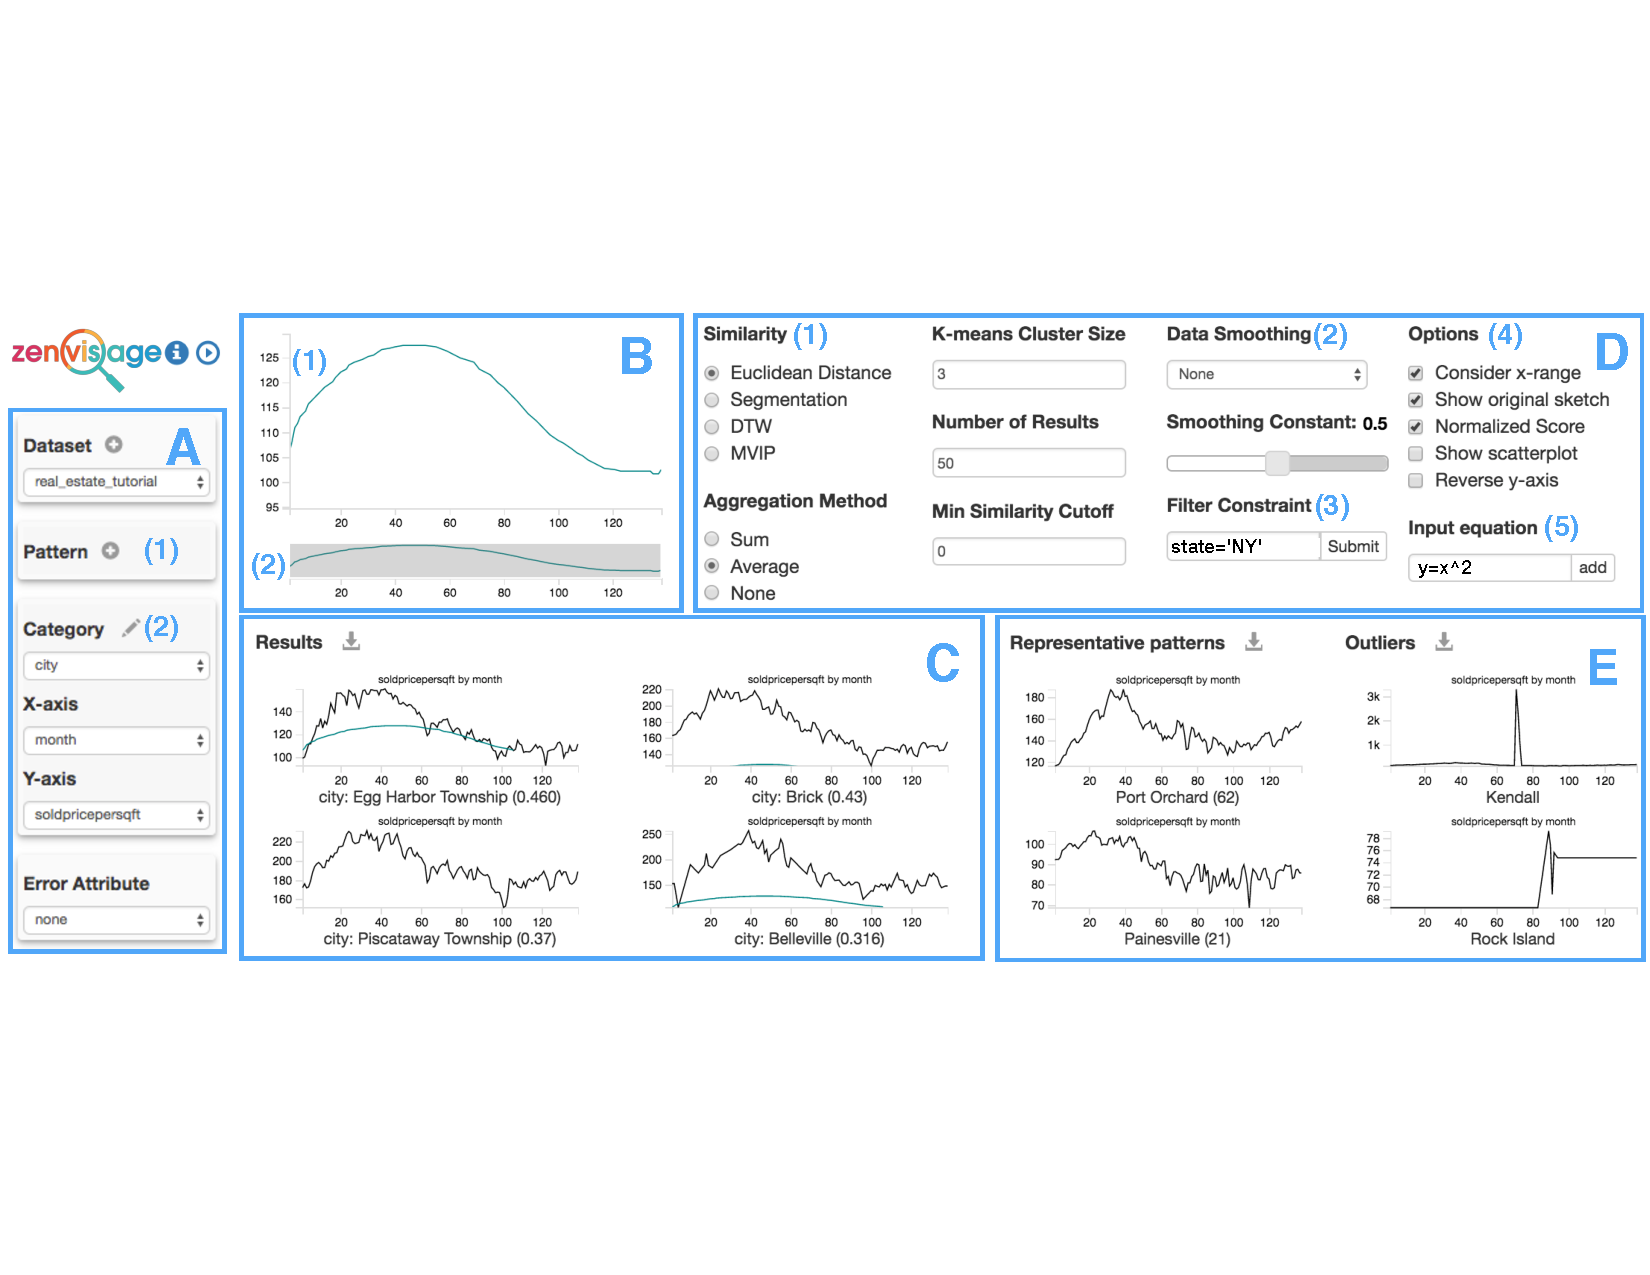
\includegraphics[width=0.9\linewidth]{figures/zvpp_system.pdf} %5.5
   \vspace{-5pt}\caption{The \zvpp system consists of : (A) data selection panel (where users can select visualized dataset and attributes), (B) query canvas (where the queried data pattern is submitted and displayed), (C) results panel (where the visualizations most similar to the queried pattern are displayed as a ranked list), (D) control panel (where users can adjust various system-level settings), and (E) recommendations (where the typical and outlying trends in the dataset is displayed).}
   \label{zvOverview}
   \vspace*{-10pt}
 \end{figure*}
 \par While our collective brainstorming led to the cross-pollination and generalization of features, this technique can also lead to unnecessary features that result in wasted engineering effort. During the design phase, there were numerous \cut{problems and associated }features proposed by participants, not all of which were incorporated. We detail the list of criteria that was used to determine whether to implement a proposed feature (including eliminating features that were nice-to-have, one-shot operations, non-essential, or required a substantially different set of research questions) in Appendix~\ref{apdx:pdartifact}. Failure to identify these early signs in the design phase may result in feature implementations that turn out not to be useful for the participants or result in feature bloat.
 \subsection{System Overview\label{sec:system}}% as described in the Figure~\ref{timeline} timeline
 The features in Table~\ref{bigfeaturetable} were incrementally incorporated and improved over time, leading to our final \cut{PD product}\rchange{prototype}, \zvpp. Given the space limitations, we will focus our discussion on the major capabilities relevant to the study findings, and defer the details of other features to the appendix and online documentation\footnote{Documentation: \url{http://github.com/zenvisage/zenvisage/wiki}}. The \zvpp interface is organized into 5 major regions all of which dynamically update upon user interactions. Typically, participants begin their analysis by selecting the dataset and attributes to visualize in the \emph{data selection panel} (Figure~\ref{zvOverview}A). Then, they specify a pattern of interest as a query (hereafter referred to as \emph{pattern query}), through either sketching, inputting an equation, uploading a data pattern, or dragging and dropping an existing visualization, displayed on the \emph{query canvas} (Figure~\ref{zvOverview}B). \zvpp performs shape-matching between the queried pattern and other possible visualizations, and returns a ranked list of visualizations that are most similar to the queried pattern, displayed in the \emph{results panel} (Figure~\ref{zvOverview}C). At any point during the analysis, analysts can adjust various system-level settings through the \emph{control panel} (Figure~\ref{zvOverview}D) or browse through the list of \emph{recommendations} provided by \zvpp (Figure~\ref{zvOverview}E). For comparison, the existing \zv system (Figure~\ref{oldZV} in Appendix~\ref{apdx:pdartifact}) from~\cite{Siddiqui2017} allowed users to query via sketching or drag-and-drop and displayed representative and outlier pattern recommendations, but had limited capabilities to navigate across different data subsets and had few control settings. Our \zvpp system is open source and available at: \url{http://github.com/zenvisage/zenvisage}. %\techreport{Our \zvpp system is open source and available at: \url{github.com/[Annonymized for Submission]}.}
 